\chapter{OPTIONS, SWAPS, FUTURES, MBSs, CDOs, AND OTHER DERIVATIVES}
\begin{chapquote}{Paul Krugman}
``By 2005 or so, it will become clear that the Internet’s impact on the economy has been no greater than the fax machine’s.''
\end{chapquote}

\section{Put and call options}
Let's say you are convinced that a company is going to perform very well in the next month and its shares will increase in value. You can either buy the stock at its current price $S$ or pay a small price $f$ to have the option to buy the same stock in the future for a strike price $S_1$ and sell it within an expiry date. In this second case, you can buy the stock when you want within the expiry date. Depending on the value $S_1$ and on the value of the stock in the future, buying the option may be better than buying the stock. In particular, if the stock has a negative trend, you may want not to buy the stock and avoid losses―other than the initial cost $f$. This is the American call option, where you can buy and sell whenever you want. In the European option instead, one can sell only at the expiry date. Comparing buying a call option with buying a stock, one notices that the call option is a leverage: From a small amount of money $f$, one can have a return on investment much higher. On the other side, the worst case is the same for both: Losing 100\% of your money, either $f$ or $S$ (even if losing $S$ means the shares become worthless and its much less likely than not buying the option).
There are two payoff diagrams that can be analyzed: the value diagram and the profit-loss diagram. In both diagrams the x-axis is the stock price at expiry date. In the first one, the y-axis is how much the option is worth:
\begin{equation}\label{eq:value_diagram_call}
            f(x) = 
    \begin{cases}
        0,                  & \text{if } x\leq S\\
        x - S,              & \text{otherwise.}
    \end{cases}
\end{equation}
We can see from equation \ref{eq:value_diagram_call} that the value is always non-negative and it's linear after $x > S$.
The second diagram embeds the notion of $f$, the initial payment for the option, but the trend is similar:
\begin{equation}\label{eq:PL_diagram_call}
            f(x) = 
    \begin{cases}
        -f,                     & \text{if } x\leq S\\
        x - S - f,              & \text{otherwise.}
    \end{cases}
\end{equation}

A put option instead gives you the right to sell the stock at a specified price $S_1$ before an expiry date. In case the stock loses its value and goes below $S_1$, say at $S_2$, you can buy the stock at $S_2$ and sell it at $S_1$ and make profit. In other words, the lower the stock value, the higher the revenue. If it does not go below $S_1$ you simply don't buy the stock and you just lose $f$. A put option is less risky than shorting because in case the price goes up, you don't risk anything. As always, less risk means less reward. Put options have an American and a European version and with a price $f$, like in a call option. Also for the put option we have more leverage compared to shorting\footnote{Remember, shorting requires a 50\% upfront payment when borrowing stocks}, but the worst case is much better (100\% loss at most). The payout functions are reported in equations \ref{eq:value_diagram_put} and \ref{eq:PL_diagram_put}. 
\begin{equation}\label{eq:value_diagram_put}
            f(x) = 
    \begin{cases}
        0,                  & \text{if } x\geq S\\
        S - x,              & \text{otherwise.}
    \end{cases}
\end{equation}
\begin{equation}\label{eq:PL_diagram_put}
            f(x) = 
    \begin{cases}
        -f,                     & \text{if } x\geq S\\
        S - x - f,              & \text{otherwise.}
    \end{cases}
\end{equation}

These previous four equations are represented in Figure~\ref{fig:diagrams1}.
\begin{figure}[h!]
\centering
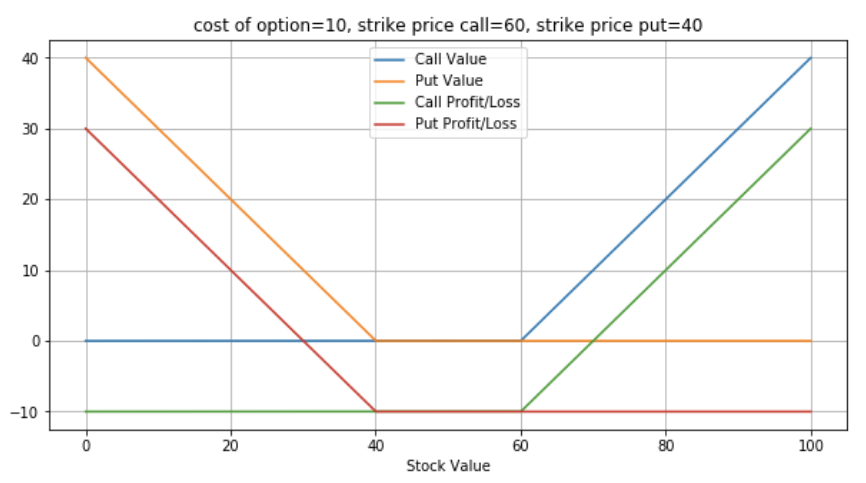
\includegraphics[width=0.8\textwidth]{images/diagrams1.png}
\caption{Value and Profit/Loss diagrams for call and put options.}
\label{fig:diagrams1}
\end{figure}

It is interesting to see what happens when one combines a stock with an option of that stock. Owning a stock can be represented simply by $f(x) = x$ in the value diagram, but by adding a put option of that stock, we get the result represented in Figure~\ref{fig:SPValue}. In Figure~\ref{fig:SPPL} the Profit/Loss diagram shows that buying a put option and the stock is like having an insurance on that stock. Ideally, you'd like to have the linear part of the green line in Figure~\ref{fig:SPPL} as close as possible to the blue line, which means a low-priced put option. The difference between the initial price of the stock and the strike price of the put option plays an important role as well.

\begin{figure}[h!]
\centering
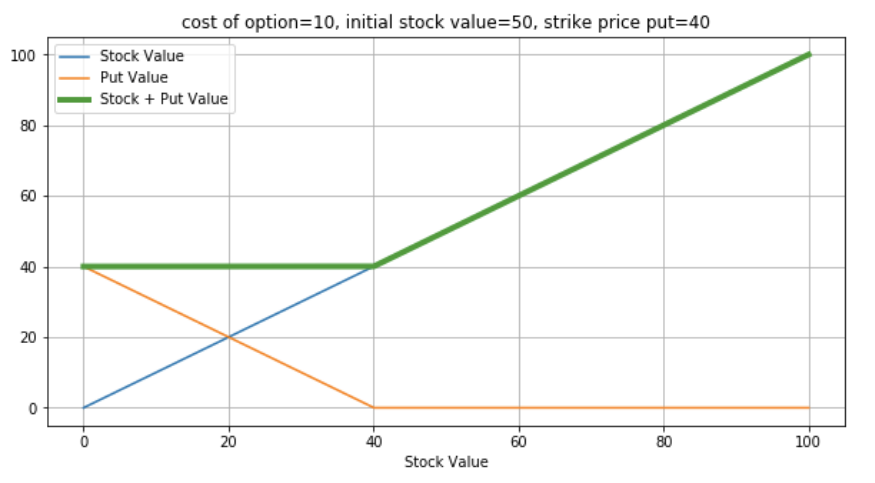
\includegraphics[width=0.8\textwidth]{images/diagrams2.png}
\caption{Stock + Put Option Value Diagram.}
\label{fig:SPValue}
\end{figure}

\begin{figure}[h!]
\centering
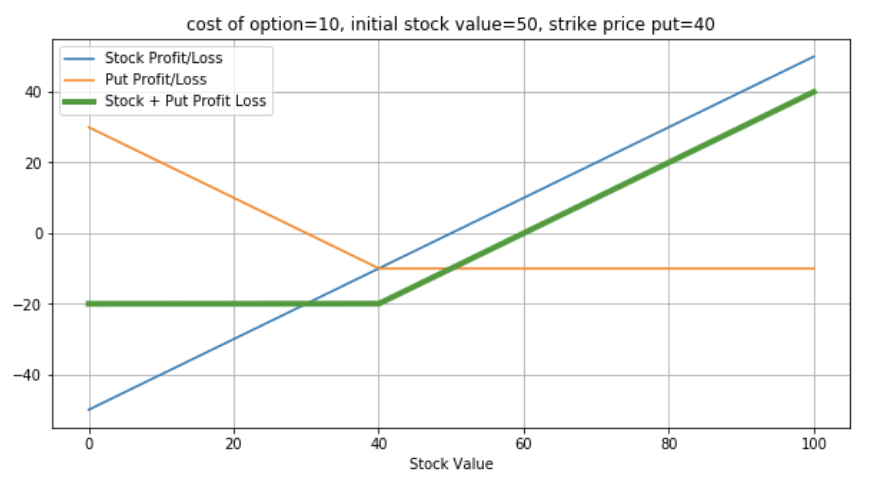
\includegraphics[width=0.8\textwidth]{images/diagrams3.png}
\caption{Stock + Put Option Profit/Loss Diagram.}
\label{fig:SPPL}
\end{figure}

What is the value diagram of a bond? Assuming we are lending money now at $S$ and getting back at maturity a sum $S_1$, regardless of the stock value, the value diagram would be a straight line parallel to the x-axis crossing the y-axis at $S_1$\footnote{What is the profit/loss diagram of a bond and a call???}. An example is shown in Figure~\ref{fig:BCValue}.
By looking at the value diagram, we can see that having a stock and a put is the same as having a bond and a call, in other words: $S + P = B + C$ and this is the so-called put/call parity. If this is not the case, there is an opportunity to make risk-free money (explained later).

\begin{figure}[h!]
\centering
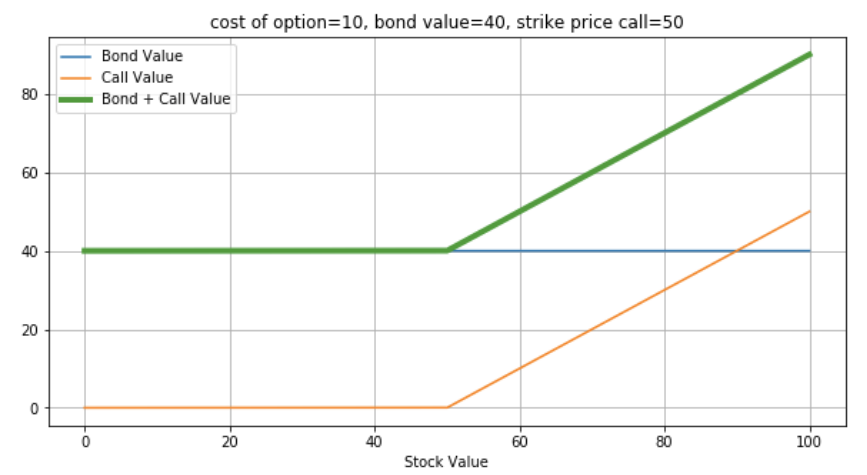
\includegraphics[width=0.8\textwidth]{images/diagrams4.png}
\caption{Bond + Call Option Value Diagram.}
\label{fig:BCValue}
\end{figure}


Owning both a put and a call option allows you to make money if you foresee a big change in value of the stock. Assuming that the P/L diagram is just a down-shift of the value diagram depending on the price of the two options, one makes profit when the stock price increases or decreases more than the price of the two options. This can be easily verified by drawing put and call P/L diagram with the same strike-price (see Figure~\ref{fig:long_straddle}).

\begin{figure}[h!]
\centering
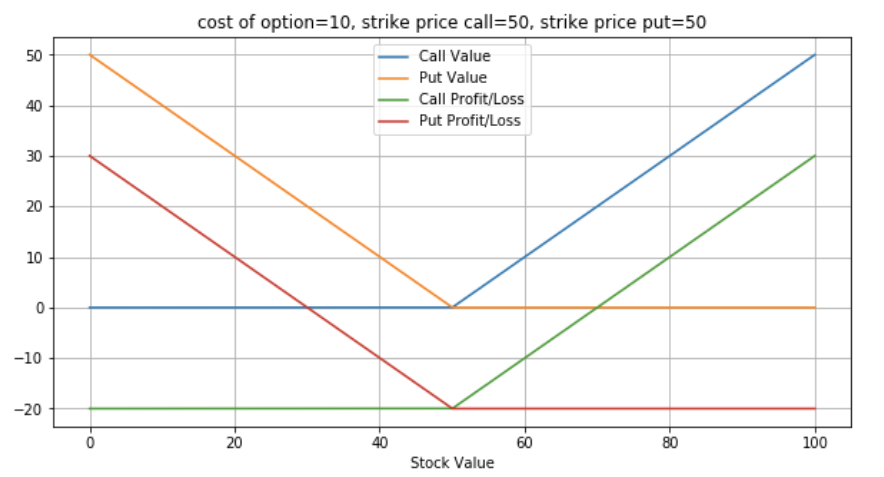
\includegraphics[width=0.8\textwidth]{images/long_straddle.png}
\caption{Long Straddle Diagram.}
\label{fig:long_straddle}
\end{figure}


If you are able to buy a call or a put option is because there is someone willing to give you the right to buy or sell in the future the stock. This person is the option writer and her value and profit/loss diagram is the mirror image ($y' = - y$) of the option holder.

Assume a stock price is $s$, its put option is trading at $p$ for a strike value $P$ and the call option is trading at $c$ for a strike value $C$. Assume also a bond you can buy at $b$ that is worth $B$ at expiry date (the same as the options) and $B = P = C$.
Now, what if $s + p > c + b$? In finance, you always buy low and sell high, so you get the call option and the bond and you sell (short) the stock and you write a put option. By doing this you immediately get money $m = s + p - c - b$. Then, at expiry date you remain with this initial profit and everything else cancels out. Let's see how from a value perspective. If the stock value goes to zero, you don't exercise the call option and it's worthless, you buy the stock at zero to cover the short, you have to buy the stock at price $P$ from the put option you wrote, but you get $B$ from the bond, hence no additional profits, nor losses, only the initial profit $m$. If the stock value goes close to zero, the stock bought with the put option can then be sold, essentially covering the short position. What if the stock price increases instead to $s_1$? You exercise the call option with a strike price $C$ and you get $s_1 - C$, you also have $B$ from the bond and you will have to cover the short by spending $s_1$ which is exactly what you have from the call and the bond,  while the put option is worthless and it won't be exercised by its owner. Similar reasoning can be done if $s + p < c + b$, in which case you buy the stock and a put option, while you write the call and sell the bond, with a profit $m = c + b - s - p$. If the stock goes to zero, you exercise the put option and get $P$, the stock is worthless and the call is not exercised by its owner, but you must pay back your bond of $B=P$. If the stock value goes to $s_1 > P$, you don't exercise the put, you have the stock which is worth $s_1$, you lose $s_1 - C$ from the call option and you pay $B$, again no profits, nor losses.

To better understand put and call options, let's examine Figure~\ref{fig:GEoptions}. Upper-left corner is the current stock price. Call options on the left, put options on the right, in the middle the strike price for both of them. Column \textit{Last} is the last trading price, \textit{Chg} is how much it changed during that day, \textit{Volume} is the number of options traded during that day, \textit{Open interest} is how may open contracts are available in the market. If you sum \textit{Last} and \textit{Strike Price}, you get a bit more than the current stock price because you have the option to buy the stock and make for money in the future, till the expiry date, which is April 2011 in this case (always the third Friday of the month). The longer the validity of the option, the higher the trading price, because you have more opportunity to make money. It is always better not to exercise the option before the expiry date, because you may lose the opportunity to make money. The best solution would be to sell it to someone, charging him this opportunity.

\begin{figure}[h!]
\centering
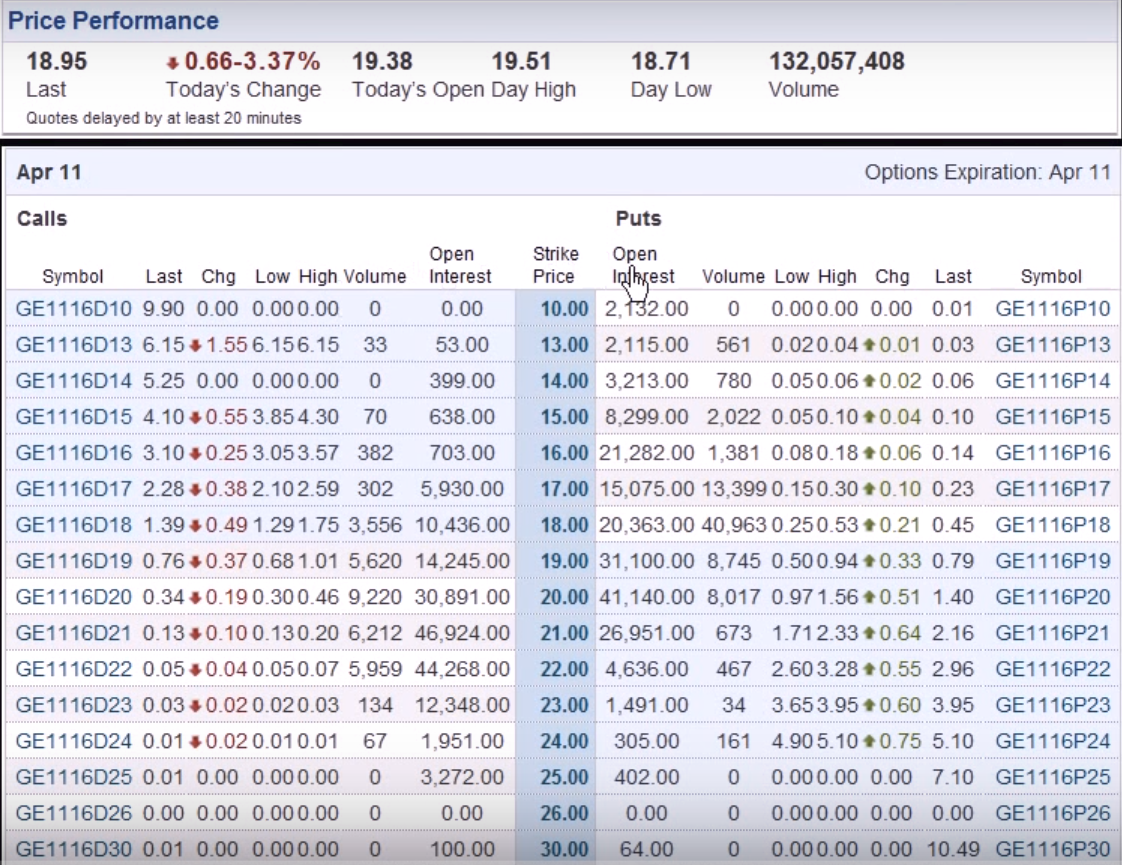
\includegraphics[width=0.8\textwidth]{images/GE_options.png}
\caption{GE call and put options.}
\label{fig:GEoptions}
\end{figure}

When a stock has a very high volatility, it is good to use put or call options as you may exercise them very easily, but their cost will go up consequently.

\section{Forward and futures contracts}
A forward contract is a document in which a seller and a buyer agree upon a certain price of a certain good or service at a specific date in the future. An example is when a farmer wants to sell apples and a food chain wants to buy them but recently the price has been very volatile depending on the good or bad season. Low price is good for the chain, high price is not, so they find an appropriate price.

What if the seller is not able to keep his promises? Or the chain goes bankrupt? What if the farmer wants to change slightly the contract, but another farmer is willing to get the old one? Future contracts are standardized forward contracts, guaranteed by an exchange and may offer more granular options on price and quantity, satisfying multiple sellers and buyers. 

How can an exchange make money out of this? Continuing the example of the farmer and the chain, the exchange will ask a certain price $p$ per Kg of apple to the chain and it will give to the farmer a sum $s < p$. Imagine now that there is another farmer willing to sell apples at a lower price $s' < s$ on a future contract and the exchange will sell this at a price $s' < s$. The aforementioned buyer will be pretty angry now because there is a cheaper option she cannot use and is tempted not to put the money at the end of the contract. To hedge this risk, the exchange asks both parties to set aside a sum, called margin, that the exchange will use in case of price oscillation of the same future contracts in the market. If there is a future contract with a cheaper price per unity of good, the exchange will take the difference from the buyer and give it to the seller. Vice versa, if the price increases the exchange will take money from the seller and put it in the buyer margin. If a margin of a party goes below a certain threshold called maintenance margin, the exchange will ask the party to put money again in its margin and go back to the original margin value. This is a mark-to-market technique because the exchange marks the price of the goods in the future contract depending on its value on the market.

A normal future curve has an increasing trend. On the x-axis we have the time for the contract to expire, and on the y-axis the value of the good. At time $t = 0$, the price is the spot price, while at $t = t'$ the curve is telling you what is the price of the good at which today you agree to buy at time $t'$. Of course this curve will not exactly follow the spot price day by day as new events may change the price. For example, if they discover a new application for silver, it's futures price will increase. An inverted curve has instead a decreasing trend and appears in particular occasions.

The size of a futures contract is a number that defines how many apples (ounces of gold, stocks or whatever the underlying asset is) will be sold/bought at expiration date. It is also known as multiplier because if the value of a stock increases by \$10, then the value of the contract will change not by a factor of 1, by a factor of $M$, the multiplier/size of the futures contract. 

\subsection{Contango}
A commodity market (in general metals or long-term investments) is in contango when it is cheaper to buy the commodity now than with a future contract. If you buy gold now, it is usually because you think in the future will value more, but buying it now has some costs: storing it somewhere safe and the cost of cash (you could have invested your money in something else). If you instead enter a future contract, you can use your money for other investments while waiting for the end of the future contract and you don't have the cost of storing.
An alternative and probably more precise definition of contango is when the commodity price agreed today to pay at contract's maturity is higher than the estimated spot price of the commodity at contract's maturity. In general, a severe contango means that the cost of financing and storing a current purchase for sale later is very high, but also that we have a surplus now or we'll have a shortage in the future.
If there is a severe contango situation, you'd buy the commodity now, enter a future contract as seller, store the commodity and sell it at maturity, making money thanks to the cheaper-than-expected costs of having the commodity. If many people start doing this it would increase the price of the commodity at the beginning and decrease it at maturity when more people will sell. This opportunity of making free money will disappear quickly as more people will spot it and eventually the future price will be equal to\footnote{We can think of it as an upper bound.} the spot price plus the cost of storing and financing (borrow money) the commodity.
From Investopedia.com: "Contango is when the futures price is above the expected future spot price. Because the futures price must converge on the expected future spot price, contango implies that futures prices are falling over time as new information brings them into line with the expected future spot price".

\subsection{Backwardation}
Backwardation is instead when the future price of the commodity is lower than the expected spot price in the future. What you should do in this case is to enter a future contract as a buyer and buy a risk-free bond that will pay you at maturity the exact amount of money needed for the future contract. This would be cheaper than buying the commodity now and storing it. Again, as soon as many people spot this opportunity of easy money, the future price will be equal to the spot price of today plus the cost of storing and the risk-free interest rate\footnote{This would be a lower bound.}. The risk-free interest rate and the loan borrowing interest rate play the role of determining the commodity's price: If they are the same rate, the price would be rational, if they are not, there would be arbitrage.
Normal backwardation is desirable for speculators who are "net long" in their positions: they want the futures price to increase.

An important note. When we say that the futures price converges to the spot price by the time we get closer to maturity time, this does not mean that a \$100 future contract will be changed to say \$80. It means that the \$20 from the margin will be sent from the buyer to the seller and the contract looks like a \$80 future, but still \$100 will be paid at maturity.

Contango and normal backwardation are just theories because you cannot be sure about the spot price of a commodity in the future, you just have an estimate. You can see though the phenomenon of contango or backwardation when futures prices are adjusted (decreasing or increasing) to the spot price.

The fair value of a futures contract is the strike price of the future contract at which the buyer is neutral between buying the stock (commodity) in the market now or in the futures market for the next expiry date. Futures markets have much longer trading hours, sometimes also 24 hours. Let's assume that a stock closed at a spot price $S$, and the corresponding fair value (in future strike price) for the next front month was $S + 2$, but now the futures market trades the same stock currently at $S+1$. This means that the spot price should be lower (around $S - 1$ to keep the same gap of 2) and as soon as the stock market will reopen, the stock value will go down as the market will sell the commodity. By having this information, one could think of taking advantage of it, but nowadays there are automated systems that look at these futures contracts and execute high-frequency trading to immediately exploit these opportunities and make money. If instead the futures price is at say $S+5$, the stock value should be higher.

\section{Mortgage-backed securities}
When someone needs a loan to buy a house, she goes to a commercial bank and gets it with some interest rate. This commercial bank will have lots of other customers with their respective loans. What this bank can do to get some immediate cash is to sell these mortgages to an investment bank with some sort of fees. This investment bank usually creates a special purpose entity (SPE) with these mortgages as assets and will try to sell shares of this company to investors hoping to sell the stocks at a higher price than what the SPE spent to buy the mortgages. These stock are called mortgage-backed securities (MBS)

\section{Collateralized debt obligations}
The MBSs can be split in different tranches. One with a lower interest rate but more secure, a mezzanine in the middle and the last is the most junior, the equity with higher interest rate but more risk. These are collateralized debt obligations.

\section{Credit default swaps}
An example to introduce credit default swaps (CDS) is the following. A pension fund, which collects pensions from people can only invest on companies with good ratings. What if it wants to borrow a sum of money $S$ to company A, which has a rating lower than the allowed threshold? The pension fund can pay a small percentage $r_{CDS}$, for example 2\% of the bond from company A with a rate $r_B$, say 10\%, to an insurance company, with a good rating, which will intervene in case of default of the company. So, the pension fund is basically getting a bond with an interest rate $r_E = r_B - r_{CDS} = 8\%$ backed by the insurance company with good ratings, but the bond itself comes from company A which has bad ratings. The insurance company can be any business as long as it has a good rating. The pension fund is buying CDS and the insurance company is selling CDS. The insurance company though is not obliged to put some money aside in case of default from company A, but the rating will change if they don't, in the long run.

Now, if some expert, e.g., a hedge fund, thinks that a company is going to default soon and wants to bet against it, it can buy a CDS without lending the money to the company (it's just a bet between CDS buyer and seller). This means that the hedge fund will pay the annual small percentage of interest rate $r_{CDS}$ to the CDS issuer to cover a sum $S$, as a normal pension fund would do, and if the company defaults, than it would get the sum $S$. The interesting part here is that the CDS buyer can bet on any sum $S$ as long as he can pay $S\cdot r_{CDS}$ every year to the CDS issuer. Of course, the CDS buyer will lose money if the company does not default. The sooner the default, the smaller the costs, the higher the profit.

The risk here is that if company A defaults, the CDS seller may be able to pay money to the buyer of company A's CDS, but what if by doing this, the CDS seller gets its ratings degraded? All the other CDS that were sold by that insurance company are now to be unwound. 
As pointed out also by Warren Buffett, the CDS system is (or at least was) dangerous for the entire financial system because an insurance company is taking bets on amounts of money far larger than what they can insure, without taking the proper countermeasures in case of actual defaults. So, the people, hedge funds for example, who thought to be insured, are now facing risk and people who were hedging on hedge funds are at risk as well.

Another example of CDS buyer is when a special-purpose entity offers CDOs and wants to get some sort of insurance on the senior tranche.

\section{Interest rate swaps}
In general there are two possible ways to decide the interest rate of a loan. The simpler is to fix it at a certain number $r_f$, the other is to keep it variable with time according to another index (e.g., LIBOR). What if someone has a fixed interest rate but would like to have a variable interest rate? And what about the opposite, someone with a variable rate that would like to fix it at a certain rate? The purpose of interest rate swaps is exactly this, to change from fix to variable and vice versa. Alice has a loan with a bank with fixed interest rate $r_f$ and Bob has a variable interest rate $r_v = LIBOR + k$, where $k$ is some non-negative constant. With a interest rate swap, Alice would pay $r_f$ to her bank plus $r_v$ to Bob, while Bob would pay $r_v$ to his bank and $r_f$ to Alice. So, net net they swapped their interests.


\section{Black-Scholes formula}
Given a certain stock price $S$, the exercise price $X$ (strike price) of its call option, its standard deviation of log returns (volatility) $\sigma$, the current risk-free interest rate $r$, the B.S. formula gives us the correct price $C$ of a European call option with a time to expiration $T$.

\begin{equation}
    \label{eq:BSformula}
    C = S \mathcal{N}(\delta_1) - X e^{-r T} \mathcal{N}(\delta_2)
\end{equation}
where:
\begin{equation}
    \delta_1 = \dfrac{\ln{\Big(\dfrac{S}{X}\Big)} + (r + \dfrac{\sigma^2}{2})T}{\sigma \sqrt{T}}
\end{equation}
\begin{equation}
    \delta_2 = \dfrac{\ln{\Big(\dfrac{S}{X}\Big)} + (r - \dfrac{\sigma^2}{2})T}{\sigma \sqrt{T}}
\end{equation}
and $\mathcal{N}(x)$ is the CDF of the normal distribution.
The input values are five: $S, X, T, r$ and $\sigma$. This last value is only the historical volatility of the stock, which is used as an estimation of its future value.
As call options are traded in the market, one can use this formula to get the implied volatility of the stock simply inverting the equation.

\section{Additional notes}

\subsection{Selling put options of bonds}
"For the second day in a row, a put option on the 30-year Treasuries futures contract was heavily sold, a sign of confidence that long-end yields won’t rise much." \citep{yield_inversion}

To me, if a put option is heavily sold, it means that the markets predict the price of the underlying asset will lose value, so that they will be able to sell the asset at the exercise price which is higher than the current strike price. Applying this to the bond market, if what I wrote above is true, they think the prices of US treasuries will be lower, which means higher interest rates. Where am I wrong? The answer is that I misinterpreted the news and what I wrote is a bit misleading. If a put option is heavily sold, the sellers think the underlying asset won't lose value, the buyer does think the asset will lose value.

